\chapter{Research results}

This chapter is devoted to the research results. For each research question, a separate section is used. 

\section{\ref{rq:what-is-change-detection} What is change-detection, and what do we want to use it for?}

\subsection{What is change?} \label{what-is-change}

Not many research papers could be found that define the word change. A clear definition of the word change can be found in a psychology paper by Rensink \cite{rensink2002change}.

\begin{quote}
    "The word change generally refers to a transformation or modification of something over time. As such, this notion presumes a nonchanging substrate on which changes are imposed. More precisely, change is defined here [the paper] as the transformation over time of a well-defined, enduring structure." (Rensink, 2002, p. 248).
\end{quote}

The definition of the word change can be translated to the language of \testar. The "well-defined, enduring structure" refers to the GUI of the system under test, whereas the "transformation over time" refers to the various version of the SUT. The "something" refers to a part of the GUI that can change like: Widget tree, the state or an action. 

Besides defining the word change, Rensink also describes the differences between changes and differences. A change is a transformation of the same 'something', whether a difference lacks the property of the same something. For example, what are the differences between two distinct SUT, or the same SUT but in two distinct environments or Internet Browsers? A limit to the change detection algorithm is that the SUT needs to be executed in the same environment; otherwise, false-positive changes can occur.

This distinction of definitions between change and differences give the first limit to this research paper's proposed change detection algorithm. The change detection algorithm will give the changes of a SUT, between versions, in the same environment since a different environment can influence the model and therefore influence the outcome of the change detection.

\subsection{What change detection?}

toool made by F-secure. collaboration with Pekka GUI Driver. both had features. 

automated masking abstract away know a lot. image comparison. 

GUITAR, something. 

F-secure change detection point it own 
new tool, no paper. 

Change what we are intresing in.

starting state depends on existng data. external changes removed. 

percent of change pixel could indicate .... div > 50\% change then different. 
1 level-> differences on the screen.
2 level-> change in the model (state graph)
3 level-> Form testing, from testing correct and incorrect form
 - hint faker library phone number etc...
 - relationship between 

find values on the new page. releation input value and one of the screen. you input phonenumber. on screen is presented on

metaphorfic testing (relationships). 

Alexander Pretengkro finding state machine. (Aho can connect).

Anomoli detection for change. most change happen on one stap. What if the it stop changes Trent, history change some... change on change detection. 
 
 source: meeting 2 dec with IVVES 
 
\section{\ref{rq:useful-detection} Which properties make a model useful for change detection?}

Dynamic are not usable since they can change without detectable reason. \cite{mulders2022Statemodel}

\section{\ref{rq:testar-config} Which \testar configuration will generate a useful model?}
\section{\ref{rq:finding-changes} How can we find changes between two models?}

Abstract Graph comparison
First the software create a ComparableGraph. A Comparable graph only contacts the nodes and edges from the abstract states and abstract actions. The data however will include data from the concrete states and actions. 

When we have a changed abstractstate, get a widgettree of one concrete state
https://www.xmlunit.org/  have a package for both java as .NET to create differences between version.

using a fast mode
the fast mode will only look into changes on the abstract level. Changes like different colours for example


\subsection{Calibration}
\subsection{Difference Engine}
\subsection{Difference Graph}


\section{\ref{rq:tooling} What tooling is available to show the detected differences?}

The solution is written outside the \testar application. Doing so makes it possible to work without the context and dependencies of \testar and allows the application to be written in a language more known by the developer. Building the application outside the \testar scope was possible because it only needed the state model data from the OrientDB graph database.

The solution is divided into two major parts. A \testar .NET server and a \testar .NET UI. As the name suggests, they are built and created in the Framework from Microsoft: .NET Core (version 6) \footnote{\url{https://dot.net}}. .NET is an open-source, cross-platform framework. An application created with .NET will run on Windows, Linux and macOS. 

\begingroup
\captionsetup{type=figure}
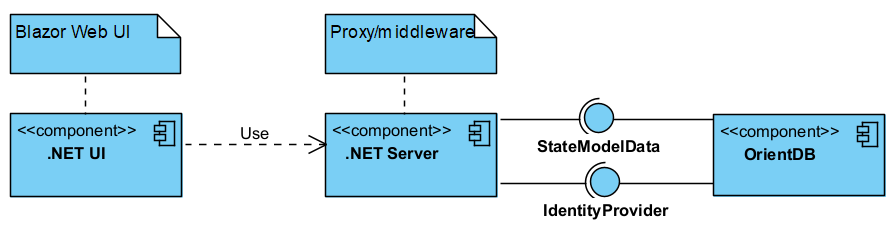
\includegraphics[scale=0.7]{thesis/images/server-ui-comp.png}
\captionof{figure}{.NET UI - Server and OrientDb component model (UML 2.0)}\label{fig:components}
\endgroup

Figure \ref{fig:components} shows the three components making up the system. The state model data that \testar generated is saved into the OrientDB graph database, the same database used by the .NET server. The .NET UI connects to the .NET server. In the following sections, the different components are explained. 

%Since both the server and the UI are running C\# code, it is possible to share the core application code in both projects. As a side benefit, the core application code can be reused in smaller applications dedicated to a single task, like change detection. 

\subsection{OrientDB Component}
OrientDB is the data storage for \testar. The created application presents the data to the user. In order to query the data, the \textsc{rest} endpoint of OrientDB is used. A \textsc{post} is sent to OrientDB with the query and parameters in the body of the request. An example of the body is displayed in listing \ref{code:example-body}.

\begin{lstlisting}[language=xml, caption=Get AbstractStateModel by the model identifier, label=code:example-body]
{
  "command": "SELECT FROM AbstractStateModel WHERE modelIdentifier = :id",
  "parameters": {
    "id": "1chdi5230521708089"
  }
}
\end{lstlisting}

An alternative way of querying the data is to use the Query \textsc{get} operation. While it is an easy way to query the data it is vulnerable to SQL injection since the parameters are directly used in the URL and can therefor be altered.

The current solution in which the queries are send from the UI to the .NET server is not completely fool proof either. It is still possible to, for example by using the Burp Suite, to alter the \textsc{post} message body and attach the OrientDB server. To circumvent this issue it would be recommended to setup a \textsc{rest} endpoints that returns data and lets the .NET server creates the SQL calls to OrientDB. 

It is not recommended to expose the OrientDB database directly to a public network \cite{orientdb-security}. To build the application with good security in mind, the database is exposed through a Proxy/middle-ware component, the .NET server. In the next section the .NET server component is explained in more detail.

\subsection{.NET Server}

The .NET Server servers as Proxy between the .NET UI component and the already existing OrientDB graph database. The only user of the .NET server is UI component. However it is possible to have other applications use to .NET Server to query data stored in OrientDB. 

The need for the .NET Server was due to browser restrictions and limitations accesing the Database. Two issues arise when the UI was trying to connect to the Database. The issue was \acrfull{cors} and it a security feature in which the server can permit or denay a request from a client if the request was not made by a trusted source \cite{cors}. By default OrientDB does not permit other websites to use the \textsc{rest} endpoints from OrientDB \cite{orientdb-webserver}. It is possible to enable to CORS in the OrientDB configuration but that would mean administrators should edit the OrientDB config before the .NET application could be used and secondly it would not fix the second issue, accessing the session cookie.

The second issue prevented the UI to read the cookie created by OrientDB. Before a user can query the data it need to sign in the OrientDB. This is accounplised by executing a \textsc{get} command to the /connect/database endpoint and provide the username and password, encoded with the base64 algorithm, as a authentication header. If the credentials are valid, the OrientDB will return a \textsc{204 ok} response with a \textsc{osessionid} in the response headers. The \textsc{osessionid} is used to authenticate the user on future calls.

It was impossible to retrieve the \textsc{osessionid} and reuse it in the data retrieval processes. Not able to save the \textsc{osessionid} resulted in saving the username and password in local storage of the browser, making it available for retrieval with a Cross Site Scripting attack. 

The OrienDB url and \testar state model data are provided in the server configuration. Based on user feedback it also possible to enable multi database feature. With that feature it becomes possible to specify the name of the database during logging in. For example, if the user wants to connect to the database \verb|TestarData| and the username is \verb|Kirk|, the username for sign in becomes: \verb|TestarData\Kirk|.

\subsection{.NET UI}
With the \testar application it is possible to open an analysis website \cite{thesisMulders}. This website provided a couple of features like viewing the viewing the state models, Test sequences and a graph engine created with Cytoscape.js. To view this analysis website the user have to install \testar on their machine. In this thesis a new website is presented, that can be used outside the \testar application. It got a fresh look and feel, created with Bootstrap\footnote{\url{https://getbootstrap.com}} and a noticeable increase in performance. Figure \ref{fig:ui-home-page} show the new available models screen. 

\begingroup
\captionsetup{type=figure}
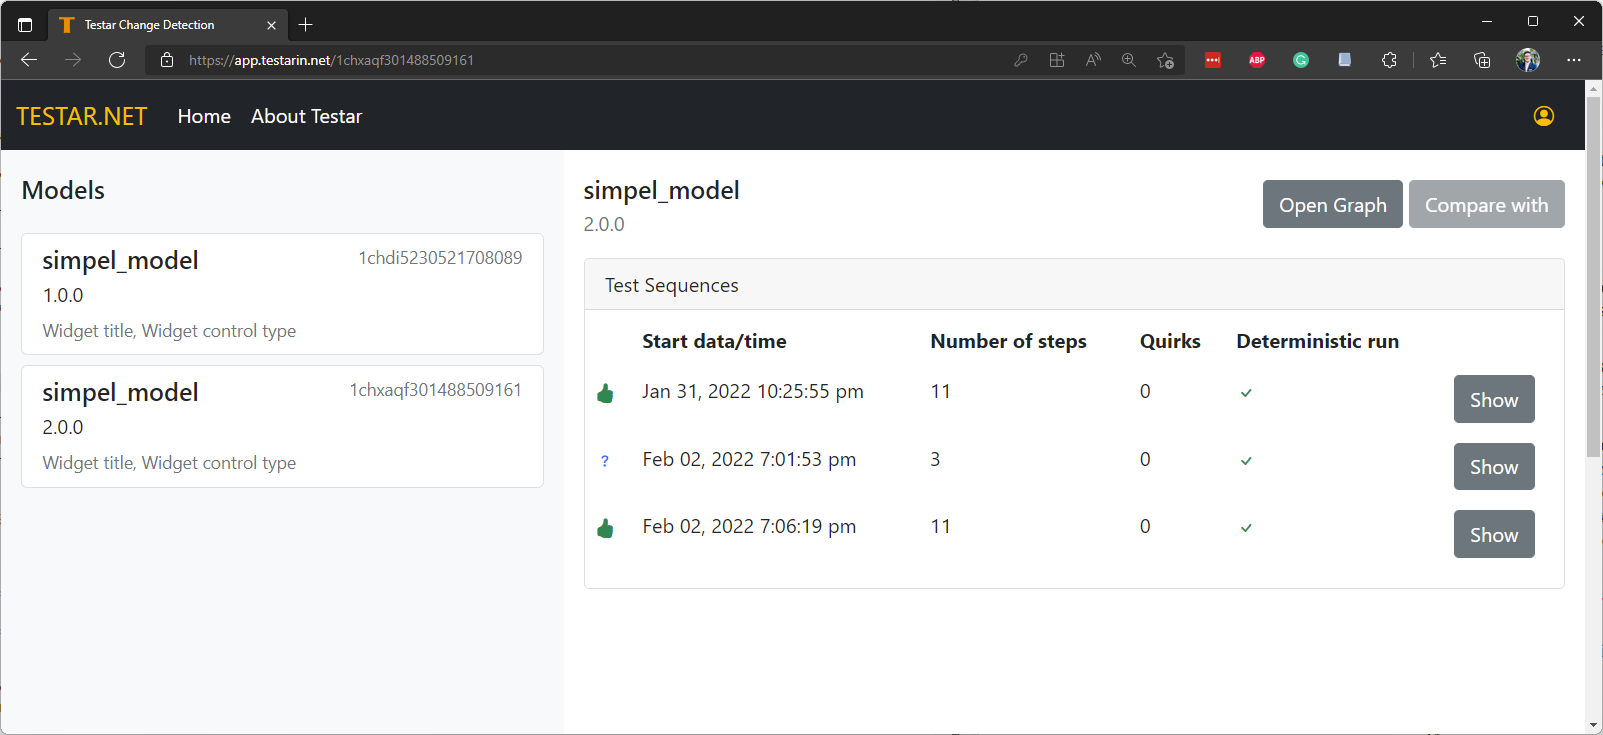
\includegraphics[scale=0.4]{thesis/images/ui-home-page.png}
\captionof{figure}{Available models in the new \testar website}\label{fig:ui-home-page}
\endgroup

The new \testar analysis website is created in Blazor. Blazor is an interactive web UI technology that allows running .NET code in the browser \cite{what-is-blazor}. For the graphical layer, Blazor uses HTML. The application code is wrtiten in C\# although some parts are still coded in Javascript. 

The code required to display the state graph, as shown in figure \ref{fig:graph-page}, has been copied from the original \testar analysis website. Beside the HTML layer and the retrieval of the raw model data, nothing has been altered. The graph engine is still using the Cytoscape library. 

\begingroup
\captionsetup{type=figure}
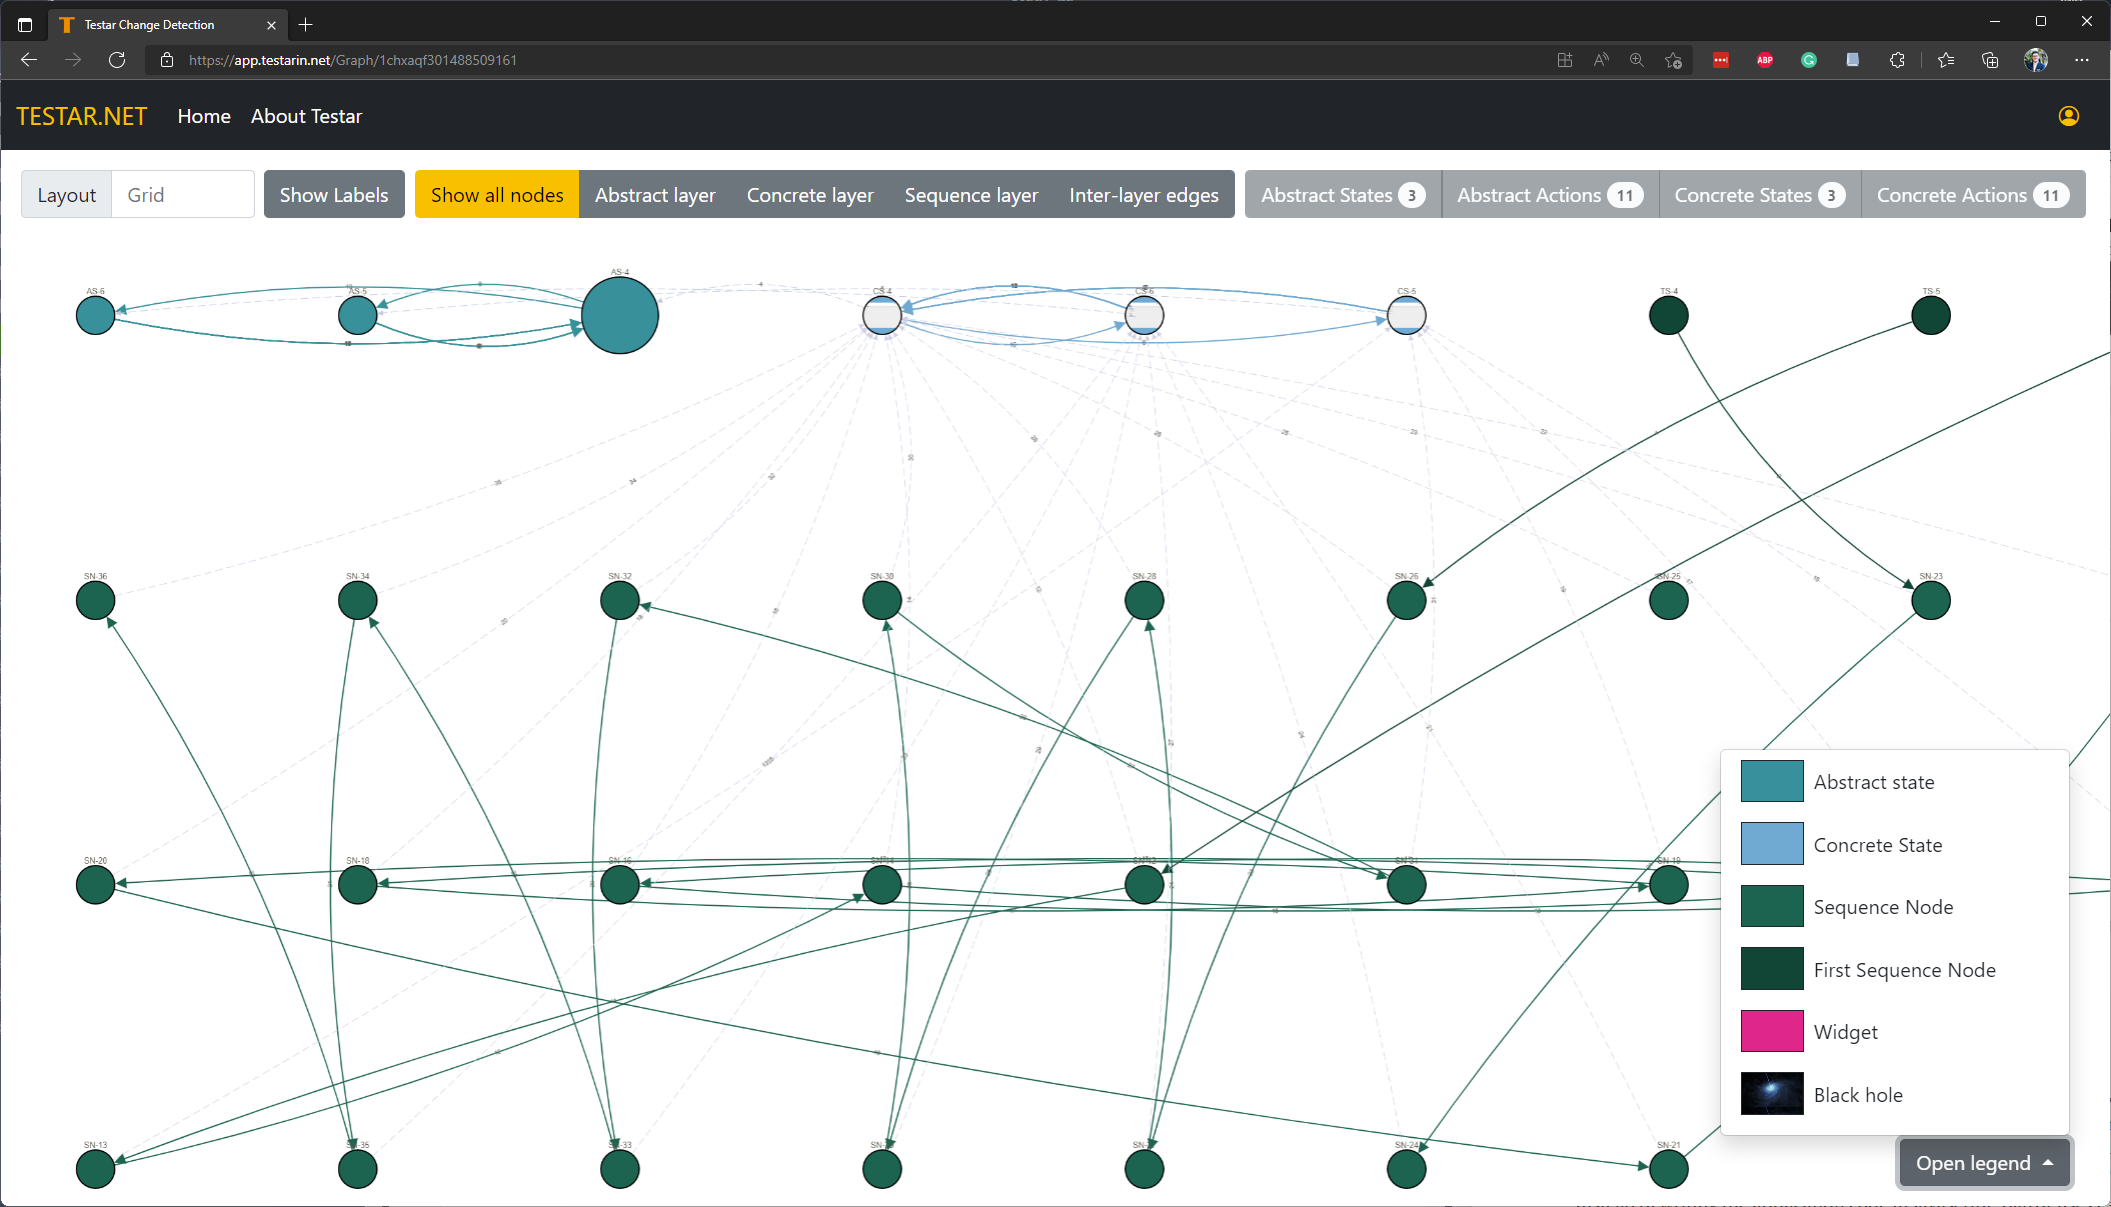
\includegraphics[scale=0.3]{thesis/images/graph-page.png}
\captionof{figure}{The new Graph page}\label{fig:graph-page}
\endgroup

\subsection{Authentication \& Authorisation}
The .NET server helps with solving the security issues but still provide a secure and open authentication endpoint. External applications that want to use the .NET endpoints must first authenticate with the .NET server upon it will return a \acrfull{jwt}. A JWT is defined as a "compact, URL-safe means of representing claims to be transferred between two parties." \cite{jones2015json}.

Before the user can use the UI it needs to authenticate itself. Figure \ref{fig:auth-sd} shows the sequence diagram how the authentication flow is handled. Since the user identities are stored in the identity provider of the graph database, it is important to note that the .NET server does neither handle authentication nor authorisation. As visible in the figure it only provides a sign in proxy and generated a JWT around the oSessionId. The authentication and authorisation is handled by the OrientDB server. When the user provides incorrect credentials, the graph database will return a \verb|401 Unauthorized| and the Server will return that status code to the UI.

\begingroup
\captionsetup{type=figure}
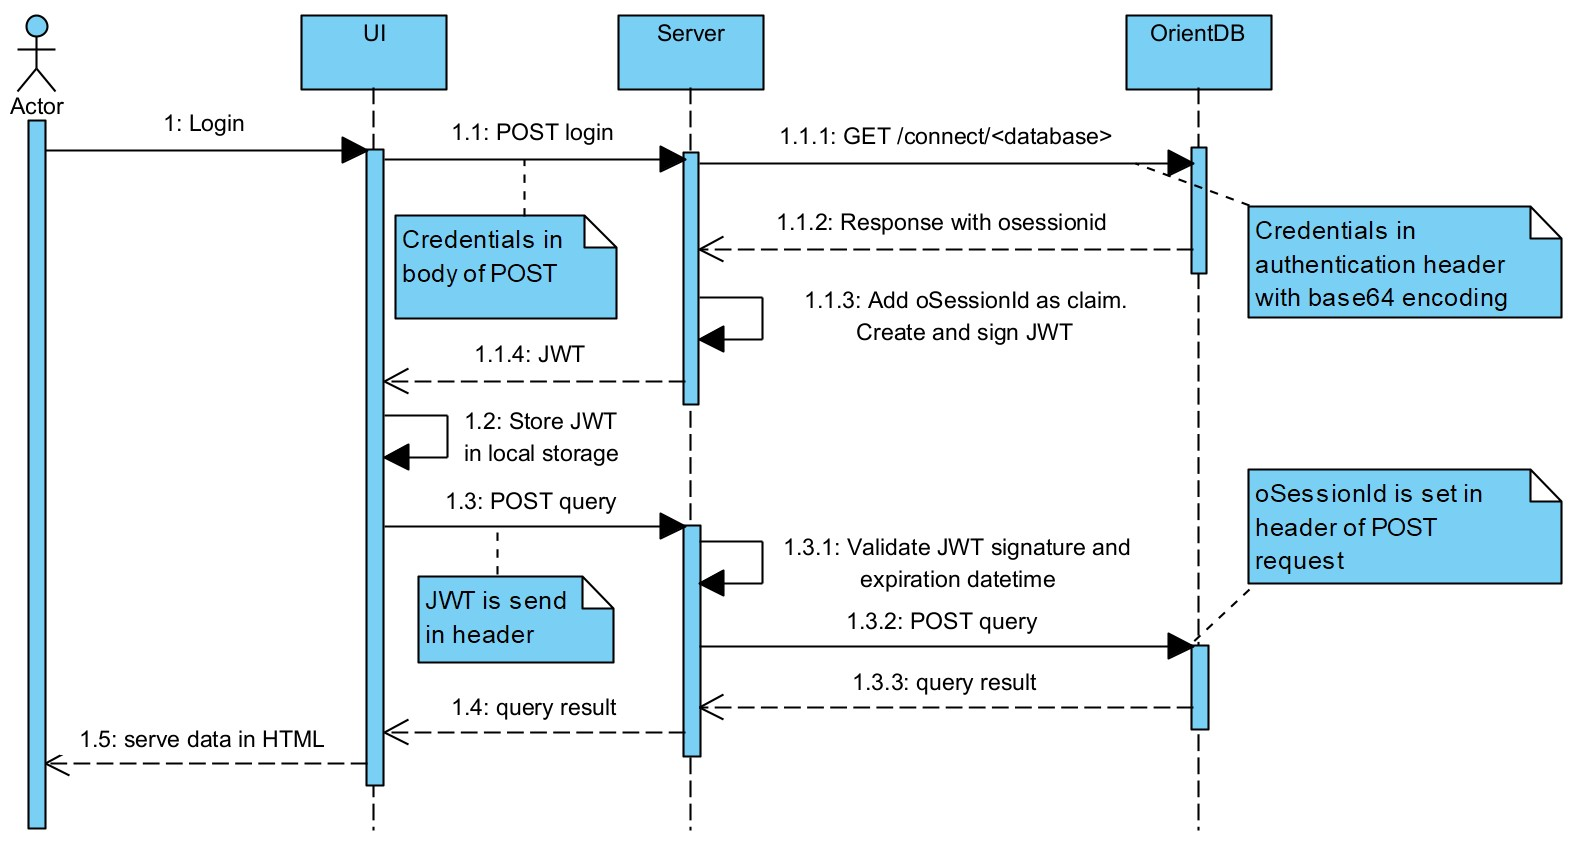
\includegraphics[scale=0.4]{thesis/images/authentication-sd.png}
\captionof{figure}{Authentication sequence (UML 2.0)}\label{fig:auth-sd}
\endgroup

An example of the JWT generated by the server is displayed in listing \ref{code:jwt}. The JWT can be decoded by anyone, for example with a website like \url{https://jwt.io}. The corresponding header and payload is displayed in listing \ref{code:jwt-payload}. In the JWT, two dots are visible which shows the different sections of the token. The first section is dedicated to the header information (lines 1-4 in listing \ref{code:jwt-payload}. The middle section contains the payload (lines 5-12 in listing \ref{code:jwt-payload}). The third and last section contains the signing information. 

\begin{lstlisting}[language=xml, caption=Example JSON Web Token (line breaks for display purposes only), style=nonrstyle, label=code:jwt]
eyJhbGciOiJIUzI1NiIsInR5cCI6IkpXVCJ9.eyJodHRwOi8v
c2NoZW1hcy54bWxzb2FwLm9yZy93cy8yMDA1LzA1L2lkZW50a
XR5L2NsYWltcy9uYW1lIjoidGVzdGFyIiwiT3JpZW50RGJTZX
NzaW9uIjoiT1NFU1NJT05JRD1PUzE2NDk3OTY5OTgxODgtMTE
3NTE5OTcxMDIyNDcxNTA0MyIsIkRhdGFiYXNlTmFtZSI6InRl
c3RhcjIiLCJleHAiOjE2NDk4MDA1OTgsImlzcyI6Imh0dHA6L
y9sb2NhbGhvc3QiLCJhdWQiOiJodHRwOi8vbG9jYWxob3N0In
0.zkSDTOuNrn9lR0ca6JLQsbSiLEskEBC_uY937q9sSU0
\end{lstlisting}

Every JWT is signed by the server (see the self-message 1.1.3 in figure \ref{fig:auth-sd}) with a secret provided during the startup of the .NET Server. With the signing information, the server can validated that it generated the JWT and that it is safe to assume the information in the payload is legit. 

There are a couple of intresting claims visible when viewing the payload. exp... by default 5 minutes. same lenght as the orientDB cookie lifetime. Line \verb|6| shows the username of the user. Line \verb|7| shows the OrientDbSession which the .NET server is using to communicate to the graph database. Line \verb|8| displayed the databasename. The databasename is only visible when on the server the feature 'MultipleDatabases' is activated. Lines \verb|9| (exp), \verb|10| (iss) and \verb|11| (aud) are showing the claims registered in the \acrfull{iana} \cite{jones2015json}. \verb|exp| Stands for 'expiration' and shows the expiration time in seconds (in Unix epoch). By default the expiration time set to 5 minutes, which is the same as the orientdb session id. 




since jwt is signed with a secret only known by the server, the server can validate whether it generated the JWT.

\begin{lstlisting}[language=xml, caption=Decoded JWT header and Payload of the JWT given in listing \ref{code:jwt}, label=code:jwt-payload]
{
  "alg": "HS256",
  "typ": "JWT"
}
{
  "http://schemas.xmlsoap.org/ws/2005/05/identity/claims/name": "testar",
  "OrientDbSession": "OSESSIONID=OS1649796998188-1175199710224715043",
  "DatabaseName": "testar2",
  "exp": 1649800598,
  "iss": "http://localhost",
  "aud": "http://localhost"
}
\end{lstlisting}



\subsection{Hosting the components}
The two new components presented in this thesis, .NET server and the \testar analysis website, need to be hosted on two individual web servers. The .NET server needs to be able to execute server side code. 

The new \testar Analysis website needs to be hosted on a web server that can host static files. Blazor is interactive by nature, but from the server's perspective, is it a static site since it does not have any server-side code execution. All code executions are handled on the user's computer. Before the user can use the website, it is downloaded on its computer before it gets executed. After the download, the application runs on the user's computer and the traffic to and from the .NET server will not travel through the public internet but stays on the local area network. 

The new \testar analysis website is publicly available on \url{https://app.testarin.net} (read as app dot \testar in dot net). The .NET server need to be hosted on the network of the user. It need to be able to access the OrientDB server. 

To help setting up the two components, two separate docker images are created. Both are available on the docker hub: \verb|rneeft/testar-net-server|\footnote{\url{https://hub.docker.com/repository/docker/rneeft/testar-net-server}} and \verb|rneeft/testar-net-ui|\footnote{\url{https://hub.docker.com/repository/docker/rneeft/testar-net-ui}}.



\section{\ref{rq:type-visualisation} How to visualise change?}

difference engine
merge graph \cite{andrews2009visual}
the graph needs to be similar are "enough"

\section{\ref{rq:shortest-set} How to generate the shortest set of actions that helps the user to reach the changed state in the SUT?}

\section{\ref{rq:req-apps} What are the requirements for validation applications?}

\section{\ref{rq:validation-apps} Which applications can be used for validation?}
